\documentclass[12pt,reqno]{amsart}
%\documentclass[../Solutions_Introduction_to_Algorithms.tex]{subfiles}
\usepackage{amsmath,amsfonts,amscd,amssymb,epsf,color,enumerate,graphicx,url}
\usepackage{algorithm, algorithmic}
\usepackage{forest, tikz, xcolor}
\usepackage{parskip}
\usetikzlibrary{matrix, positioning}
\usetikzlibrary{positioning,arrows.meta}
\setlength{\oddsidemargin}{-0.2in}%
\setlength{\evensidemargin}{-0.2in}%
\setlength{\textwidth}{6.6in}%
\setlength{\topmargin}{-0.5in}%
 \setlength{\textheight}{9.5in}%
 \definecolor{orange}{rgb}{1,0.5,0}
 \pagestyle{plain}
\linespread{1.3}
\usepackage[small]{caption}
\newcommand{\pa}{\partial}
\newcommand{\va}{\vspace{0.4cm}}
\newcommand{\di}{\displaystyle}
\newcommand{\disp}{\displaystyle}


% turn on \answertrue to show the solution
% turn on \answerfalse to hide the solution
\newif\ifanswer
\answertrue
%\answerfalse



\begin{document}
\noindent {\footnotesize Introduction to Algorithms}\hspace{10.5cm} {\footnotesize Solutions}

\vspace{0.5cm}
\hspace{5.5cm}\textbf{\large Exercises in Section 2.3}
\vspace{0.5cm}

\begin{enumerate}[1.]

\item Using Figure~2.4 as a model, illustrate the operation of merge sort on an array initially containing the sequence $\langle 3, 41, 52, 26, 38, 57, 9, 49 \rangle$.
\vspace{0.5cm}

\ifanswer
\noindent {\bf Solution}

\begin{center}
    \begin{tikzpicture}[>=Stealth,scale=1]
        
    \foreach \i in {1,2,3,4,5,6,7,8}{
    \fill[orange!25] (\i,0) rectangle ++(1,1);
    }
    \foreach \i/\v in {1/3,2/41,3/52,4/26,5/38,6/57,7/9,8/49}{
    \draw (\i,0) rectangle ++(1,1);
    \node at (\i+0.5,0.5) {\v};
    \node[above] at (\i+0.5,1) {\small \i};
    }
    \foreach \j/\v in {1/$p$,4/$q$,8/$r$}{
    \node[above] at (\j+0.5,1.5) {\small \v};
    }
    \draw[->,orange,thick] (4,-0.5) to (3,-1.5);
    \draw[->,orange,thick] (6,-0.5) to (7,-1.5);
    \end{tikzpicture}\\


    \begin{tikzpicture}[>=Stealth,scale=1]
        
    \foreach \i in {1,2,3,4,9,10,11,12}{
    \fill[orange!25] (\i,0) rectangle ++(1,1);
    }
    \foreach \i/\v in {1/3,2/41,3/52,4/26,9/38,10/57,11/9,12/49}{
    \draw (\i,0) rectangle ++(1,1);
    \node at (\i+0.5,0.5) {\v};
    }
    \foreach \i in {1,2,3,4} \node[above] at (\i+0.5,1) {\small \i};
    \foreach \i in {5,6,7,8} \node[above] at (\i+4.5,1) {\small \i};
    \foreach \j/\v in {1/$p$,2/$q$,4/$r$,9/$p$,10/$q$,12/$r$}{
    \node[above] at (\j+0.5,1.5) {\small \v};
    }
    \draw[->,orange,thick] (2,-0.5) to (1,-1.5);
    \draw[->,orange,thick] (4,-0.5) to (5,-1.5);
    \draw[->,orange,thick] (10,-0.5) to (9,-1.5);
    \draw[->,orange,thick] (12,-0.5) to (13,-1.5);
    \end{tikzpicture}\\


    \begin{tikzpicture}[>=Stealth,scale=1]
        
    \foreach \i in {1,2,5,6,9,10,13,14}{
    \fill[orange!25] (\i,0) rectangle ++(1,1);
    }
    \foreach \i/\v in {1/3,2/41,5/52,6/26,9/38,10/57,13/9,14/49}{
    \draw (\i,0) rectangle ++(1,1);
    \node at (\i+0.5,0.5) {\v};
    }
    \foreach \i in {1,2} \node[above] at (\i+0.5,1) {\small \i};
    \foreach \i in {3,4} \node[above] at (\i+2.5,1) {\small \i};
    \foreach \i in {5,6} \node[above] at (\i+4.5,1) {\small \i};
    \foreach \i in {7,8} \node[above] at (\i+6.5,1) {\small \i};
    \foreach \j/\v in {1/\text{$p,q$},2/$r$,5/\text{$p,q$},6/$r$,9/\text{$p,q$},10/$r$,13/\text{$p,q$},14/$r$}{
    \node[above] at (\j+0.5,1.5) {\small \v};
    }
    \foreach \i in {1,2,3,4}{
    \draw[->,orange,thick] (4*\i-2.5,-0.5) to (4*\i-3,-1.5);
    \draw[->,orange,thick] (4*\i-1.5,-0.5) to (4*\i-1,-1.5);
    }
    \end{tikzpicture}\\


    \begin{tikzpicture}[>=Stealth,scale=1]
        
    \foreach \i in {1,3,5,7,9,11,13,15}{
    \fill[orange!25] (\i,0) rectangle ++(1,1);
    }
    \foreach \i/\v in {1/3,3/41,5/52,7/26,9/38,11/57,13/9,15/49}{
    \draw (\i,0) rectangle ++(1,1);
    \node at (\i+0.5,0.5) {\v};
    }
    \foreach \i in {1,2,3,4,5,6,7,8}{
        \node[above] at (2*\i-0.5,1) {\small \i};
    }
    \foreach \j/\v in {1,3,5,7,9,11,13,15}{
    \node[above] at (\j+0.5,1.5) {\small \text{$p,r$}};
    }
    \foreach \i in {1,2,3,4}{
    \draw[->,orange,thick] (4*\i-2.5,-0.5) to (4*\i-2,-1.5);
    \draw[->,orange,thick] (4*\i-0.5,-0.5) to (4*\i-1,-1.5);
    }
    \end{tikzpicture}\\


    \begin{tikzpicture}[>=Stealth,scale=1]
        
    \foreach \i in {1,2,5,6,9,10,13,14}{
    \fill[orange!25] (\i,0) rectangle ++(1,1);
    }
    \foreach \i/\v in {1/3,2/41,5/26,6/52,9/38,10/57,13/9,14/49}{
    \draw (\i,0) rectangle ++(1,1);
    \node at (\i+0.5,0.5) {\v};
    }
    \foreach \i in {1,2} \node[above] at (\i+0.5,1) {\small \i};
    \foreach \i in {3,4} \node[above] at (\i+2.5,1) {\small \i};
    \foreach \i in {5,6} \node[above] at (\i+4.5,1) {\small \i};
    \foreach \i in {7,8} \node[above] at (\i+6.5,1) {\small \i};
    \foreach \j/\v in {1/\text{$p,q$},2/$r$,5/\text{$p,q$},6/$r$,9/\text{$p,q$},10/$r$,13/\text{$p,q$},14/$r$}{
    \node[above] at (\j+0.5,1.5) {\small \v};
    }
    \foreach \i in {1,2}{
    \draw[->,orange,thick] (8*\i-2,-0.5) to (8*\i-3,-1.5);
    \draw[->,orange,thick] (8*\i-6,-0.5) to (8*\i-5,-1.5);
    }
    \end{tikzpicture}\\


    \begin{tikzpicture}[>=Stealth,scale=1]
        
    \foreach \i in {1,2,3,4,9,10,11,12}{
    \fill[orange!25] (\i,0) rectangle ++(1,1);
    }
    \foreach \i/\v in {1/3,2/26,3/41,4/52,9/9,10/38,11/49,12/57}{
    \draw (\i,0) rectangle ++(1,1);
    \node at (\i+0.5,0.5) {\v};
    }
    \foreach \i in {1,2,3,4} \node[above] at (\i+0.5,1) {\small \i};
    \foreach \i in {5,6,7,8} \node[above] at (\i+4.5,1) {\small \i};
    \foreach \j/\v in {1/$p$,2/$q$,4/$r$,9/$p$,10/$q$,12/$r$}{
    \node[above] at (\j+0.5,1.5) {\small \v};
    }
    \draw[->,orange,thick] (3,-0.5) to (4,-1.5);
    \draw[->,orange,thick] (11,-0.5) to (10,-1.5);
    \end{tikzpicture}\\

    
    \begin{tikzpicture}[>=Stealth,scale=1]

    \foreach \i in {1,2,3,4,5,6,7,8}{
    \fill[orange!25] (\i,0) rectangle ++(1,1);
    }
    \foreach \i/\v in {1/3,2/9,3/26,4/38,5/41,6/49,7/52,8/57}{
    \draw (\i,0) rectangle ++(1,1);
    \node at (\i+0.5,0.5) {\v};
    \node[above] at (\i+0.5,1) {\small \i};
    }
    \foreach \j/\v in {1/$p$,4/$q$,8/$r$}{
    \node[above] at (\j+0.5,1.5) {\small \v};
    }
    \end{tikzpicture}\\




    \vspace{0.5cm}
\end{center}

\vspace{1cm}



\item The test in line 1 of the \textsc{Merge-Sort} procedure reads ``if $p \ge r$'' rather than
``if $p \ne r$.'' If \textsc{Merge-Sort} is called with $p > r$, then the subarray
$A[p\!:\!r]$ is empty. Argue that as long as the initial call of
\textsc{Merge-Sort}$(A,1,n)$ has $n \ge 1$, the test ``if $p \ne r$'' suffices to
ensure that no recursive call has $p > r$.

\vspace{0.5cm}

\ifanswer
\noindent {\bf Solution}

We need to show that $p \leq r$ in every call of \textsc{Merge-Sort}. In the initial call, $p = 1$ and $r = n$. Given $A$ is nonempty ($n \geq 1$), $p \leq r$.

Now, suppose $p \leq r$ at the start of an iteration, \textsc{Merge-Sort} is recursively called if and only if $p < r$ (therefore $p \leq r - 1$). We have $$q = \lfloor (p + r)/2 \rfloor \geq \lfloor p \rfloor = p,$$ and $$q = \lfloor (p + r)/2 \rfloor \leq \lfloor ((r - 1) + r)/2 \rfloor = \lfloor r - 1/2 \rfloor = r - 1.$$ Hence, in both recursive calls there is $p \leq r$.

\vspace{1cm}



\item State a loop invariant for the \textbf{while} loop of lines 12--18 of the
\textsc{Merge} procedure. Show how to use it, along with the \textbf{while}
loops of lines 20--23 and 24--27, to prove that the \textsc{Merge} procedure is
correct.

\vspace{0.5cm}

\ifanswer
\noindent {\bf Solution}

\textbf{Loop Invariant:} At the start of each iteration, elements from index $p$ to $p + i + j - 1$ are sorted, and are smaller than or equal to elements from index $p + i + j$ to $r - 1$.

\textbf{Initialization:} At the start of the first iteration, $i + j = 0$. Vacuously true.

\textbf{Maintenance:} Assume the loop invariant holds for an iteration. Since both $L$ and $R$ are sorted, the smaller element of $L[i]$ and $R[j]$ is smaller than all unsorted elements, and by assumption larger than all sorted elements.

\textbf{Termination:} Elements from index $p$ to $p + i + j - 1$ are sorted, with $i = n_L - 1$ or $j = n_R - 1$.

Along with the \textbf{while} loops of lines 20--23 and lines 24-27, elements from index $p$ to $r - 1$ are sorted, yielding the correctness of the \textsc{Merge} procedure.

\vspace{1cm}



\item Use mathematical induction to show that when $n \ge 2$ is an exact power of 2,
the solution of the recurrence
\[
T(n) =
\begin{cases}
2, & \text{if } n = 2,\\[6pt]
2T(n/2) + n, & \text{if } n > 2
\end{cases}
\]
is $T(n) = n \lg n$.

\vspace{0.5cm}

\ifanswer
\noindent {\bf Solution}

Suppose $n = 2^k$ for some $k \ge 1$.

\textbf{Base case:} If $k = 1$, $T(2) = 2 = 2 \lg 2$.

\textbf{Inductive step:} Assume $T(2^k) = 2^k \lg 2^k$. Then, \begin{align*} T(2^{k+1}) &= 2T(2^k) + 2^{k+1}\\ &= 2(2^k \lg 2^k) + 2^{k+1}\\ &= 2^{k+1} \lg 2^k + 2^{k+1}\\ &= 2^{k+1} \lg 2^{k+1}. \end{align*}

\vspace{1cm}



\item You can also think of insertion sort as a recursive algorithm. In order to sort
$A[1\!:\!n]$, recursively sort the subarray $A[1\!:\!n-1]$ and then insert $A[n]$
into the sorted subarray $A[1\!:\!n-1]$. Write pseudocode for this recursive
version of insertion sort. Give a recurrence for its worst-case running time.


\vspace{0.5cm}

\ifanswer
\noindent {\bf Solution}

\begin{algorithm}
    \caption{\textsc{Insertion-Sort}$(A, n)$}
    \begin{algorithmic}[1]
        \IF{$n = 1$}
            \RETURN
        \ENDIF
        \STATE \textsc{Insertion-Sort}$(A, n - 1)$
        \STATE $key = A[n]$
        \STATE $i = n - 1$
        \WHILE{$i > 0$ and $A[i] < key$}
            \STATE $A[i+1] = A[i]$
            \STATE $i = i - 1$
        \ENDWHILE
        \STATE $A[i+1] = key$
    \end{algorithmic}
\end{algorithm}

\[
T(n) =
\begin{cases}
c_1, & \text{if } n = 1,\\[6pt]
T(n-1) + c_2n + c_3, & \text{if } n > 1.
\end{cases}
\]

\vspace{1cm}



\item Referring back to the searching problem (see Exercise 2.1--4), observe that if the
subarray being searched is already sorted, the searching algorithm can check the
midpoint of the subarray against $v$ and eliminate half of the subarray from further
consideration. The \emph{binary search} algorithm repeats this procedure, halving the
size of the remaining portion of the subarray each time. Write pseudocode, either
iterative or recursive, for binary search. Argue that the worst-case running time of
binary search is $\Theta(\lg n)$.


\vspace{0.5cm}

\ifanswer
\noindent {\bf Solution}

\begin{algorithm}
    \caption{\textsc{Binary-Search}$(A, n, x)$}
    \begin{algorithmic}[1]
        \STATE $low = 1$
        \STATE $high = n$
        \WHILE{$low \le high$}
            \STATE $mid = (low + high)/2$
            \IF{$A[mid] = x$}
                \RETURN $mid$
            \ELSIF{$A[mid] > x$}
                \STATE $high = mid - 1$
            \ELSE
                \STATE $low = mid + 1$
            \ENDIF
        \ENDWHILE
        \RETURN -1
    \end{algorithmic}
\end{algorithm}

\[
T(n) =
\begin{cases}
c_1, & \text{if } n = 1,\\[6pt]
T(n/2) + c_2, & \text{if } n > 1.
\end{cases}
\]

There are roughly $\lg n$ recursive calls, so the running time is $c_2\lg n + c_1 = \Theta(\lg n)$.

\vspace{1cm}



\item The \textbf{while} loop of lines 5--7 of the \textsc{Insertion-Sort} procedure in Section~2.1
uses a linear search to scan (backward) through the sorted subarray $A[1\!:\!j-1]$.
What if insertion sort used a binary search (see Exercise~2.3--6) instead of a linear
search? Would that improve the overall worst-case running time of insertion sort to
$\Theta(n \lg n)$?

\vspace{0.5cm}

\ifanswer
\noindent {\bf Solution}

No. Even we use binary search, we still need to iterate $i - 1$ times to place $key$ to the correct place in the worst case.

Extra explanation: Even you use linked list instead of array, the complexity is still $\Theta(n^2)$. That is because binary search does not work for linked list.

\vspace{1cm}



\item Describe an algorithm that, given a set $S$ of $n$ integers and another integer $x$,
determines whether $S$ contains two elements that sum to exactly $x$.
Your algorithm should take $\Theta(n \lg n)$ time in the worst case.

\vspace{0.5cm}

\ifanswer
\noindent {\bf Solution}

First, sort $S$ using binary search. Time complexity: $\Theta(n \lg n)$.

Then, for each $i$, find $x - S[i]$ using binary search. Time complexity: $\Theta(n \lg n)$.

\vspace{1cm}




\end{enumerate}

\end{document}



